\documentclass[twocolumn,showpacs,
  nofootinbib,aps,superscriptaddress,
  eqsecnum,prd,notitlepage,showkeys,10pt]{revtex4-1}
\usepackage{amsmath}
\usepackage{graphicx}
\usepackage{dcolumn}
\usepackage{hyperref}
\usepackage{float}
\usepackage{subfigure}
\usepackage{todo}
\begin{document}

\title{Traversability Estimation with Dynamic Graph CNN}
\author{Francesco Saverio Zuppichini}
% \affiliation{Universita della Svizzera Italiana (USI), Lugano}
\begin{abstract}
  Recent deep learning breakthrough have allowed to effective classify and segment point clouds by convert them into graph and feed them to \emph{Geometric Deep Learning} models. Point clouds are able to represent any shape in space making them one of the most versatile data-structure for non-euclidean dataset. The architecture that archives \emph{state of the art} results in booth classify and segment those cloud is Dynamic Graph CNN \cite{dgcnn}. It utilizes a special Convolution operator applied directly on the graph's edge called \emph{EdgeConv} using booth local and global information. The aim of this project is to first reproduce the results on the famous ModelNet40 \cite{shapenet} dataset with more than ten thousand meshed. Reproducing the paper's results ensure our architecture's correctness.
  Then, we test DGCNN against a vanilla CNN on a dataset composed by heightmaps, images where each pixel is the height value of a terrain region, labeled as traversable or not traversable. Those images were generated letting a legged crocodile-like robot, \emph{Krock}, walking into a simulated environment on synthetic maps and cropping the corresponding terrain patch around each stored trajectory pose. This dataset represents
   a really interesting playground to explore with architecture is able to extract the most information from the geometry of the terrain and correctly predict their traversability. 
\end{abstract}s
\maketitle
\section{Introduction}

Graphs can express a wide array of data structures using a set of nodes and the relationship between them, edges. Graphs are non-euclidean data, thus standard deep learning methods, like CNN \cite{cnn}, fails. Recently, a new set of machine learning models, \emph{Graph Deep Learning} have flourished and successfully applied on a wide array of graphs structure such as social networks \todo{add cite}, proteins \todo{add cite}, and on point clouds. A Point cloud is a set of data points in space that often represents a specific 3D object by defined its points coordinates. They are extremely flexible and can be easily gather using consumer hardware such as a Kinect or a Lidar. Even if they are not graphs by definition, we can easily convert them connecting to each point $k$ neighbors.

As with images, we are interested in classify of segment those point clouds. The current architecture that achieves the \emph{state of the art} in those tasks is \emph{Dynamic Graph CNN} proposed by Wang et all \cite{dgcnn}. It utilizes a special convolution layer,  \emph{EdgeConv}, to classify or segment point clouds. 

This this project will focus on explain, test and evaluate this architecture. First, we will reproduce the results of the original paper on the classification task. Then to test its effectiveness on predicting traversability estimation using ground's patches for a legged robot by comparing it to a classic CNN approach. The discussion will only scrape the surface of the topic and will not treat in detail other architectures. If interested, we suggest to the reader the review by Zhou et all \cite{1812.08434}.
\subsection{Model}
In this section we summarized the original paper's architecture, starting by the backbone of DGCNN, the \emph{EdgeConv}.
\subsection{Dynamic Graph CNN}
Dynamic Graph CNN is composed by multiple layer of \emph{EdgeConv} stacked one after the other similar to how Convolution are integrated into CNN. Figure \ref{fig : DGCNN} shows the two architecture proposed by the Authors, for classification and segmentation. 
\begin{figure*}
  \centering
  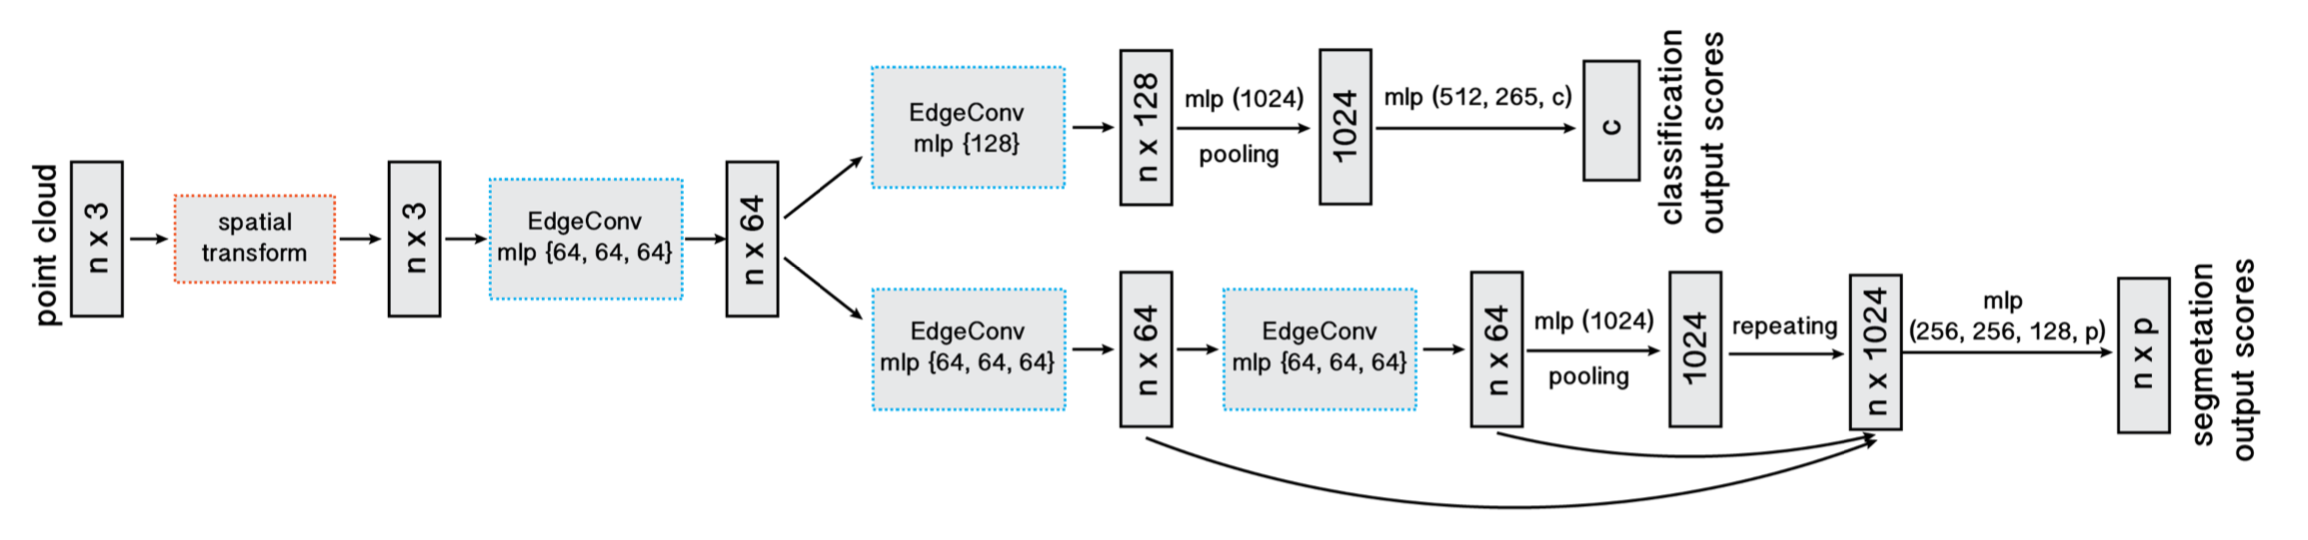
\includegraphics[width=\linewidth]{images/DGCNN.png}
\caption{The two Dynamic Graph CNN architectures divided into upper and lower branch for classification and segmentation respectively, image from the original paper \cite{dgcnn}. In each edge conv, mlp$\{n_0, ..., n_{i}\}$ represents the number of output neurons of each dense layer. For example, in the first edge conv there are three dense layers with outputs size of $64$.}
\label{fig : DGCNN}
\end{figure*}
\subsubsection{EdgeConv}
Given a point cloud with $n$ denoded as $X=\left\{x_{1}, \ldots, x_{n}\right\} \subseteq R^{F}$ and a graph $\mathcal{G}=(\mathcal{V}, \mathcal{E})$ representing the local structure of the cloud, the $i$-th output of \emph{EdgeConv} operation is defined as
\begin{equation}
  x_{i}^{\prime}=\square_{j :(i, j) \in \mathcal{E}} h_{\Theta}\left(x_{i}, x_{j}\right)
  \end{equation}
Where $\square$ is a channel wise aggregation function and $h_{\Theta}$ is the edge function. The authors choose $\square=max$ and $h_{\Theta} = h_{\Theta}(x_i, x_j - x_i)$. Where $x_i$ and $x_j$ are the coordinates of the center of the patch and its neighbors respectively. Intuitivelly, this allows the layer to use booth global and local information about the mesh. In addition, the edge function has a learnable parameter $\Theta$ that is a classic feed-forward neural network. 
\subsubsection{Dynamic EdgeConv}
\subsection{Similarties to other architectures}
% Interesting if we take an image and we convert into a graph where each node has the pixel value and there is a local connectivity between them. Then the EdgeConv becomes the classic convolution:

% \begin{equation}
%   x_{i}^{\prime}=\sum_{j :(i, j) \in \mathcal{E}} \theta_{j} x_{j}
%   \end{equation}

The authors shown that DGCNN is related to booth two categories of approaches: PointNet and graph CNN.
First, PointNet is just a special case of DGCNN where $k=1$ resulting in an empty graphs where the edge convolution functions utilises only the global information of each patch, $h_{\Theta} = h_{\Theta}(x_i)$
PointNet++ \cite{1706.02413} tries to compensate the lack of local informations by appling PointNet in a local manner, it uses a farthest point sampling algorithm to sample from the graph at each layer reducing its size at each step.

The commmon denominator with graph CNN methods, MoNet \cite{monet}, ECC \cite{ecc} and Graph Attention Network \cite{gat} and DGCNN is the notion of local patch. Hovewer, one crucial different is that all previous models work on a \emph{static} graph.


\section{Experiments}
\subsection{Setup}
We train the DGCNN classifier, up branch in figure \ref{fig : DGCNN}, on Ubuntu workstation with an nvidia TITAN-X GPU kindly borrow by the course stuff. We used \href{https://pytorch.org/}{PyTorch} and \href{https://rusty1s.github.io/pytorch_geometric/build/html/index.html}{PyTorch Geometric} to implement the tested networks. 
\subsection{Mesh Classification}
Exactly as in the original paper, we tested the model's score on the \emph{ModelNet40} dataset, a collection of more than ten thousand CAD meshed. The samples are divided into $9,843$ for training $2,468$ for testing with 40 categories. Figure \ref{fig : modelnet} shows some of the meshed for the category \emph{chair}. We randomly sampled $1024$ points from the train set and we data augmentation the points by randomly rotate and scale them. We minimized the Cross Entropy loss using Adam \cite{adam} for a total of $50$ epochs with a starting learning rate of $0.001$ reducing it each $10$ epoches by a factor of $0.2$. 
We initialised the feed forward weights  using xavier normal \cite{xavier}  and the bias to $0$. The batchnorm's weights and bias to $1$ and $0$ respectively. 
\begin{figure}[H]
  \centering
  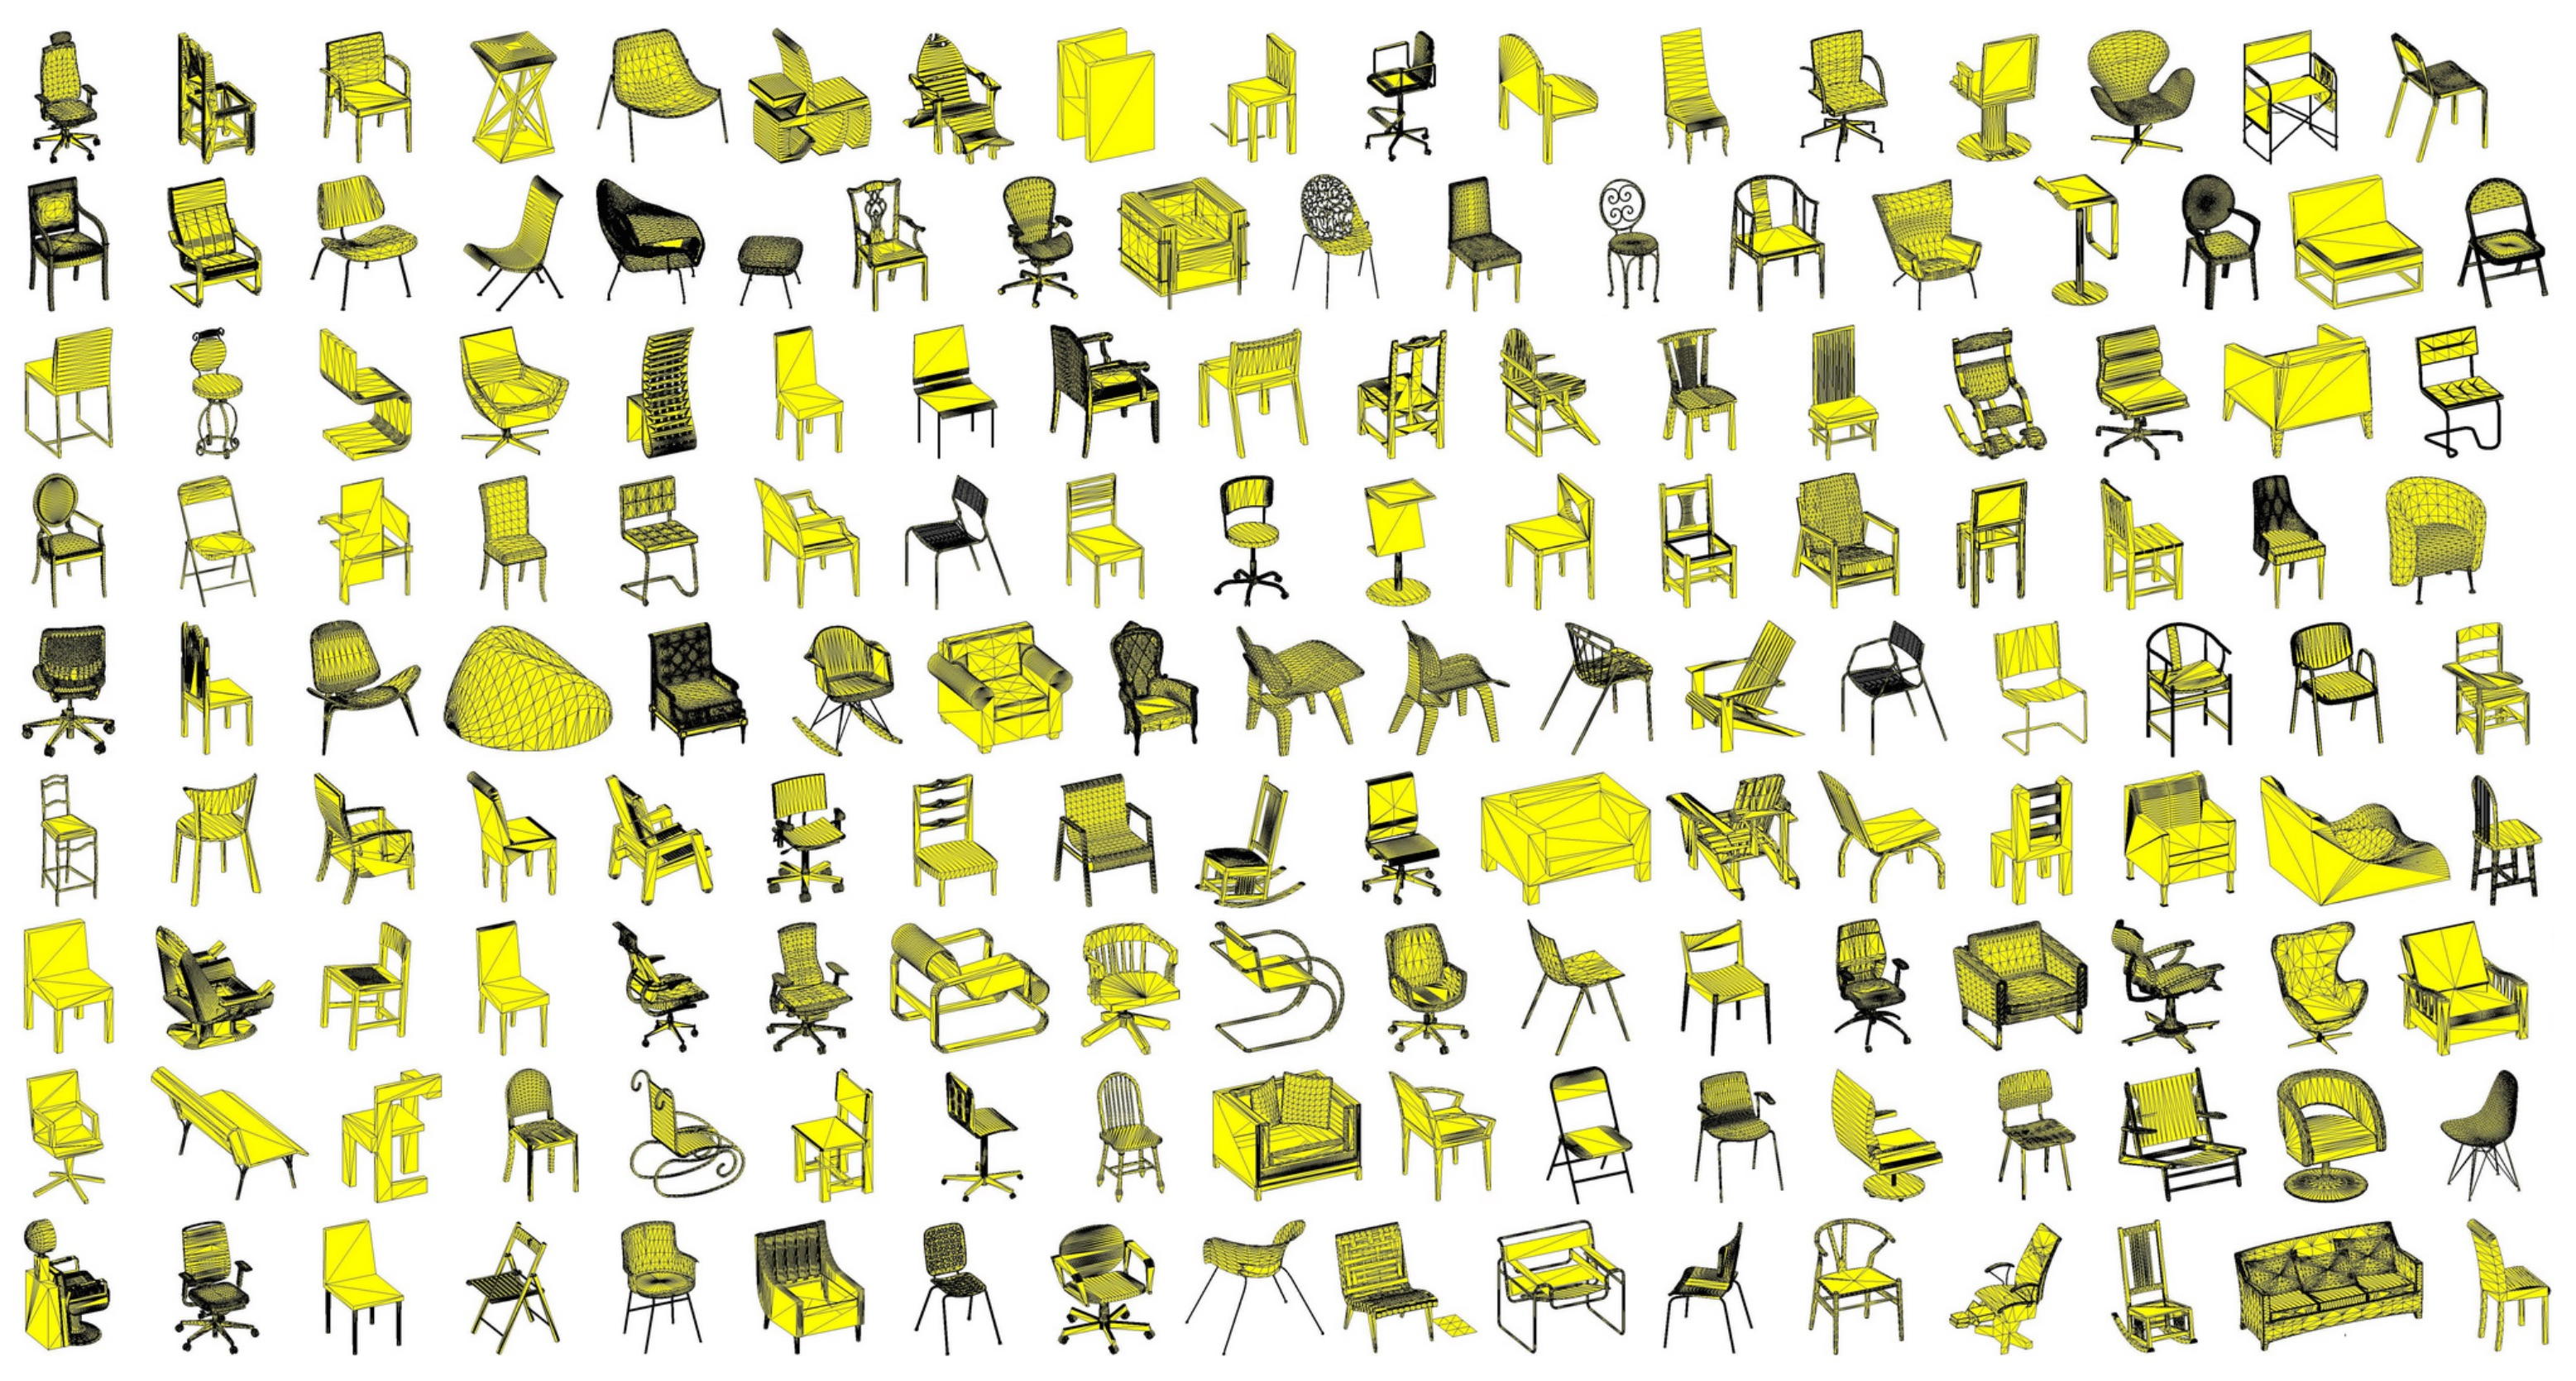
\includegraphics[width=\linewidth]{images/ModelNet.jpg}
\caption{Some of the \emph{chairs} CAD meshed in ModelNet40 \cite{shapenet}.}
\label{fig : modelnet}
\end{figure}
\subsection{Traversability Estimation}
\section{Results}
\subsubsection{ModelNet40}
The following table shows the result of the ModelNet40 dataset comparing the original DGCNN and our implementation

\begin{table}[H]
  \centering
  \begin{tabular}{lcc}
    & ACCURACY \\
    \hline
    Original & $92.2$\%  \\
    Ours & $92.1$\%  \\
    \hline
  \end{tabular}
  \caption{Test accuracy score of the original DGCNN and ours implementation on the MonelNet40 dataset.}
\end{table}
\subsubsection{Traversability Estimation}

\section{Conclusion}
We successfully reproduced the results of the original on the MonelNet40 reimplemmenting DGCNN entirely in PyTorch 
\newpage
\bibliography{bib}
\end{document}